\begin{theorem}
	Następujące warunki są równoważne: \begin{enumerate}
		\item f jest przepływem maksymalnym
		\item W sieci przepływowej nie istnieje ścieżka powiększająca od źródła do ujścia
		\item Przekrój (S,T) taki, że S zawiera wszystkie wierzchołki do których istnieje ścieżka powiększająca od źródła, jest poprawnie zdefiniowanym przekrojem, spełniającym warunek \(f(S,T) = c(S,T)\)        \end{enumerate}
\end{theorem}

\begin{proof}
	Trzeci warunek brzmi strasznie, ale tak naprawdę taki nie jest. Zajmijmy się poszczególnymi implikacjami celem udowodnienia równoważności:
	\begin{enumerate}
		\item \((1) \implies (2)\): Trywialne do udowodnienia, gdyby \(f\) było przepływem maksymalnym a istniałaby ścieżka powiększająca od źródła do ujścia to mógłbym zwiększyć wartość przepływu o 1 za jej pomocą, a więc przepływ ten nie byłby maksymalny.
		\item \((2) \implies (3)\): Ładnie się to dowodzi, stosując dowód przez rysowanie. Idea generalnie jest taka, że poprawność przekroju podanego w \((3)\) wynika nam z tego, że z \((2)\) mamy że nie istnieje ścieżka powiększająca od źródła do ujścia, a więc ujście na pewno będzie \(T\). Źródło na pewno będzie w \(S\), oczywiście. Pozostałe warunki dla przekroju oczywiście będą spełnione, więc mamy że \((S,T)\) to poprawnie zdefiniowany przekrój. Jak teraz sobie spojrzymy na wszystkie krawędzie wchodzące i wychodzące z \(S\) to odkrywamy, że skoro nie ma ścieżki powiększającej która wychodziłaby poza \(S\), to wszystkie krawędzie wychodzące muszą być w pełni wysycone, a wszystkie wchodzące wyzerowane (inaczej moglibyśmy dorzucić wierzchołek z \(T\) do \(S\), zgodnie z definicją naszego przekroju). No a skoro tak jest, to mamy że \(f(S,T) = c(S,T)\); innymi słowy przepływ przez przekrój jest równy jego przepustowości.

		      \begin{figure}[H]
			      \centering
			      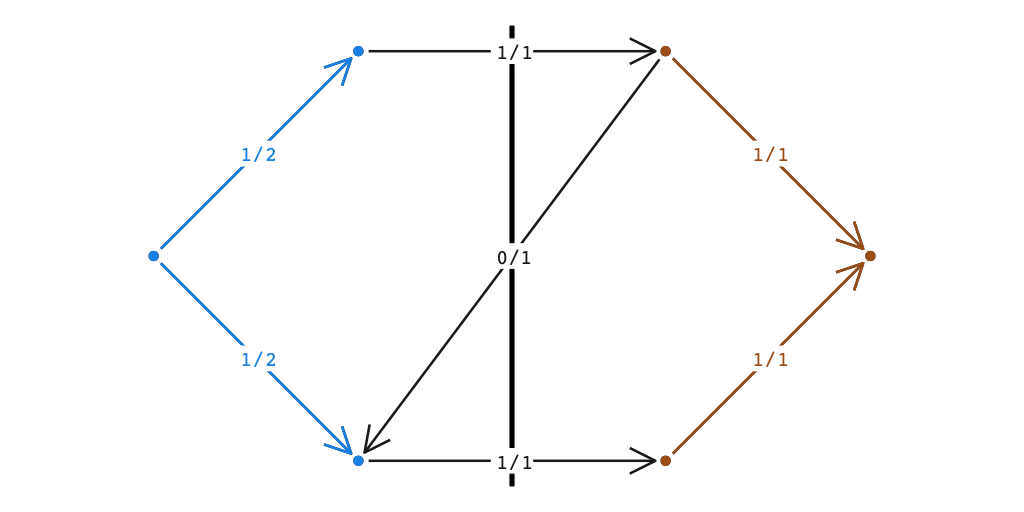
\includegraphics[scale=0.45]{images/max_flow_min_cut.png}
			      \caption{Przekrój \((S,T)\) taki, że do \(S\) należą wszystkie wierzchołki, do których idzie ścieżka powiększająca (zaznaczone na niebiesko). Nie jest możliwe poprowadzenie ścieżki powiększającej dalej, a więc krawędzie albo są maksymalnie wysycone (jeśli idą z \(S\) do \(T\)) albo wyzerowane (jeśli idą z \(T\) do \(S\)) (zaznaczone na czarno).}
		      \end{figure}

		\item \((3) \implies (1)\): Ponieważ \(val(f)\) musi być mniejsze niż przepustowość dowolnego przekroju, co zauważyliśmy już przy etapie definicji pojęć (a formaliści mam nadzieję że już dowiedli, o ile nadal nie zastanawiają się co to jest liczba parzysta), a z \((3)\) mamy, że przekrój \((S,T)\) spełnia \(f(S,T) = c(S,T)\) to mamy że przepływ ten jest maksymalny (no w sensie większego przepływu nam się nie uda zrobić, skoro właśnie osiągnęliśmy limit).

	\end{enumerate}



	Z powyższego dowodu oczywiście również wynika, że przepustowość minimalnego przekroju jest równa \(val(f)\).
\end{proof}
